\chapter{序論}
\label{chap_intro}

% 英語で言うところのイントロダクションです。通常、「序論」(introduction)で始める場合は「結論」(conclusion)という章で締めます。もし「はじめに」で始まる場合は「おわりに」です。

% この章では研究の背景や課題などを簡潔に説明します。2から4ページもあれば十分ですし、細かく節に分ける必要もありません。この章で必要なことは、なぜこの論文が書かれたのか、過去の研究に対する位置付け・課題は何か、この研究でどこまでを明らかにしようとしているのかを少ないページ数で説明することです。

% このような序論の存在しない修士論文はたくさん存在しますが、何十ページにもなる修士論文では研究の位置付けや課題がどこに書かれているのか読者は見失いやすくなります。先頭に独立した章で簡潔に道筋を示すことで、続く章を読者が読みやすくなります。

\section{素粒子標準模型}
\label{sec_intro_sm}
素粒子標準模型は物質を構成する基本粒子である素粒子とそれらの間に働く相互作用を記述した理論体系である。標準模型を構成する素粒子は 17 種類あり、物質を構成するフェルミオン、相互作用を媒介するゲージボゾン、質量の起源となるヒッグス粒子に分けられる。
表\ref{tab:fermion}にフェルミオンの性質をまとめる。フェルミオンは強い相互作用をしないレプトンと、強い相互作用をするクォークに分けられ、それぞれ3世代6種類の素粒子で構成される。
% Please add the following required packages to your document preamble:
% \usepackage{multirow}
\begin{table}[]
    \centering
    \caption[標準模型のフェルミオン]{標準模型のフェルミオン}
    \label{tab:fermion}

    \begin{tabular}{ccccccc}
    \hline
                                               &                                            & 名称        & 表記           & 質量                 & 電荷   & スピン \\ 
    \hline\hline
    \multicolumn{1}{c|}{\multirow{6}{*}{クォーク}} & \multicolumn{1}{c|}{\multirow{2}{*}{第1世代}} & アップ       & $u$            & 2.2 MeV            & +2/3 & 1/2 \\
    \multicolumn{1}{c|}{}                      & \multicolumn{1}{c|}{}                      & ダウン       & $d$            & 4.7 MeV            & -1/3 & 1/2 \\ \cline{2-7}
    \multicolumn{1}{c|}{}                      & \multicolumn{1}{c|}{\multirow{2}{*}{第2世代}} & チャーム      & $c$            & 1.3 GeV            & +2/3 & 1/2 \\
    \multicolumn{1}{c|}{}                      & \multicolumn{1}{c|}{}                      & ストレンジ     & $s$            & 93 MeV             & -1/3 & 1/2 \\ \cline{2-7}
    \multicolumn{1}{c|}{}                      & \multicolumn{1}{c|}{\multirow{2}{*}{第3世代}} & トップ       & $t$            & 173 GeV            & +2/3 & 1/2 \\
    \multicolumn{1}{c|}{}                      & \multicolumn{1}{c|}{}                      & ボトム       & $b$            & 4.2 GeV            & -1/3 & 1/2 \\ \cline{2-2}
    \hline\hline
    \multicolumn{1}{c|}{\multirow{6}{*}{レプトン}} & \multicolumn{1}{c|}{\multirow{2}{*}{第1世代}} & 電子ニュートリノ  & $\nu_{e}$    & < 2 eV     & 0    & 1/2 \\
    \multicolumn{1}{c|}{}                      & \multicolumn{1}{c|}{}                      & 電子        & $e$            & 511 keV            & -1   & 1/2 \\ \cline{2-7}
    \multicolumn{1}{c|}{}                      & \multicolumn{1}{c|}{\multirow{2}{*}{第2世代}} & ミューニュートリノ & $\nu_{\mu}$  & < 0.19 MeV & 0    & 1/2 \\
    \multicolumn{1}{c|}{}                      & \multicolumn{1}{c|}{}                      & ミューオン     & $\mu$        & 106 MeV            & -1   & 1/2 \\ \cline{2-7}
    \multicolumn{1}{c|}{}                      & \multicolumn{1}{c|}{\multirow{2}{*}{第3世代}} & タウニュートリノ  & $\nu_{\tau}$ & < 18.2 MeV & 0    & 1/2 \\
    \multicolumn{1}{c|}{}                      & \multicolumn{1}{c|}{}                      & タウ        & $\tau$       & 1.78 GeV           & -1   & 1/2 \\ \hline
    \end{tabular}
\end{table}

表1.2にボゾンの性質をまとめる。ボゾンは強い相互作用を媒介するグルーオン、弱い相互作用を媒介するWボゾンとZボゾン、電磁相互作用を媒介する光子などのゲージボゾンと質量の起源であるヒッグス粒子で構成されている。

\begin{table}[]
    \centering
    \caption[標準模型のフェルミオン]{標準模型のフェルミオン}
    \label{tab:bozon}

    \begin{tabular}{cccccc}
    \hline
                                                                                           & 名称        & 表記           & 質量                 & 電荷   & スピン \\ 
    \hline\hline
    \multicolumn{1}{c|}{\multirow{4}{*}{ベクターボゾン}}  & グルーオン       & $g$            & 0            & 0 & 1 \\
    \multicolumn{1}{c|}{}                                            &   W ボゾン     & $W^{+}$            & 80.4 GeV            & $\pm$1 & 1 \\ 
    \multicolumn{1}{c|}{}                       & Z ボゾン      & $Z^{0}$           & 91.2 GeV            & 0 & 1 \\
    \multicolumn{1}{c|}{}                                            & 光子    & $\gamma$            & 0             & 0 & 1 \\
    \hline\hline
    \multicolumn{1}{c|}{\multirow{1}{*}{スカラーボゾン}}  & ヒッグス  & $h$    & 125 MeV     & 0    & 0 \\
    \hline
    \end{tabular}
\end{table}


素粒子標準模型は現在まで多くの実験によって高い精度で検証されているものの、天文観測から明らかになった暗黒物質の存在やヒッグス粒子の質量に対する階層性問題など多くの問題点を内包している。これらの問題を体系的に解決する理論として、標準模型の素粒子とスピンが1/2異なるパートナー粒子を導入する超対称性理論が有力視されており、その直接的な検証は素粒子物理学の最重要課題である。一般に超対称性粒子は大きな質量を持っていることが知られ、加速器を用いたエネルギーフロンティア実験は超対称性の検証に向けた重要な役割を果たす。
\section{LHC-ATLAS実験}
\label{sec_intro_atlas}

ジュネーブに拠点を置く欧州原子核研究機構(CERN)では、超対称性粒子をはじめとする新粒子探索や素粒子標準模型の精密測定を目的としてLHC-ATLAS実験を行なっている。
LHCはスイスとフランスの国境付近に設置された陽子陽子衝突型加速器で、その周長は26.7 kmに及ぶ(図\ref{LHCoverview})。LHCには8つの地下と地上をつなぐトンネルがあり、それぞれPoint1からPoint8と名付けられている。このうち4つのPointで陽子陽子衝突が行われ、各衝突点ではそれぞれ特徴の異なる検出器を用いた独立した実験が行われている。本研究はその中の一つであるA Toroidal LHC ApparatuS (ATLAS)実験に関するものである。

\begin{figure} 
\centering
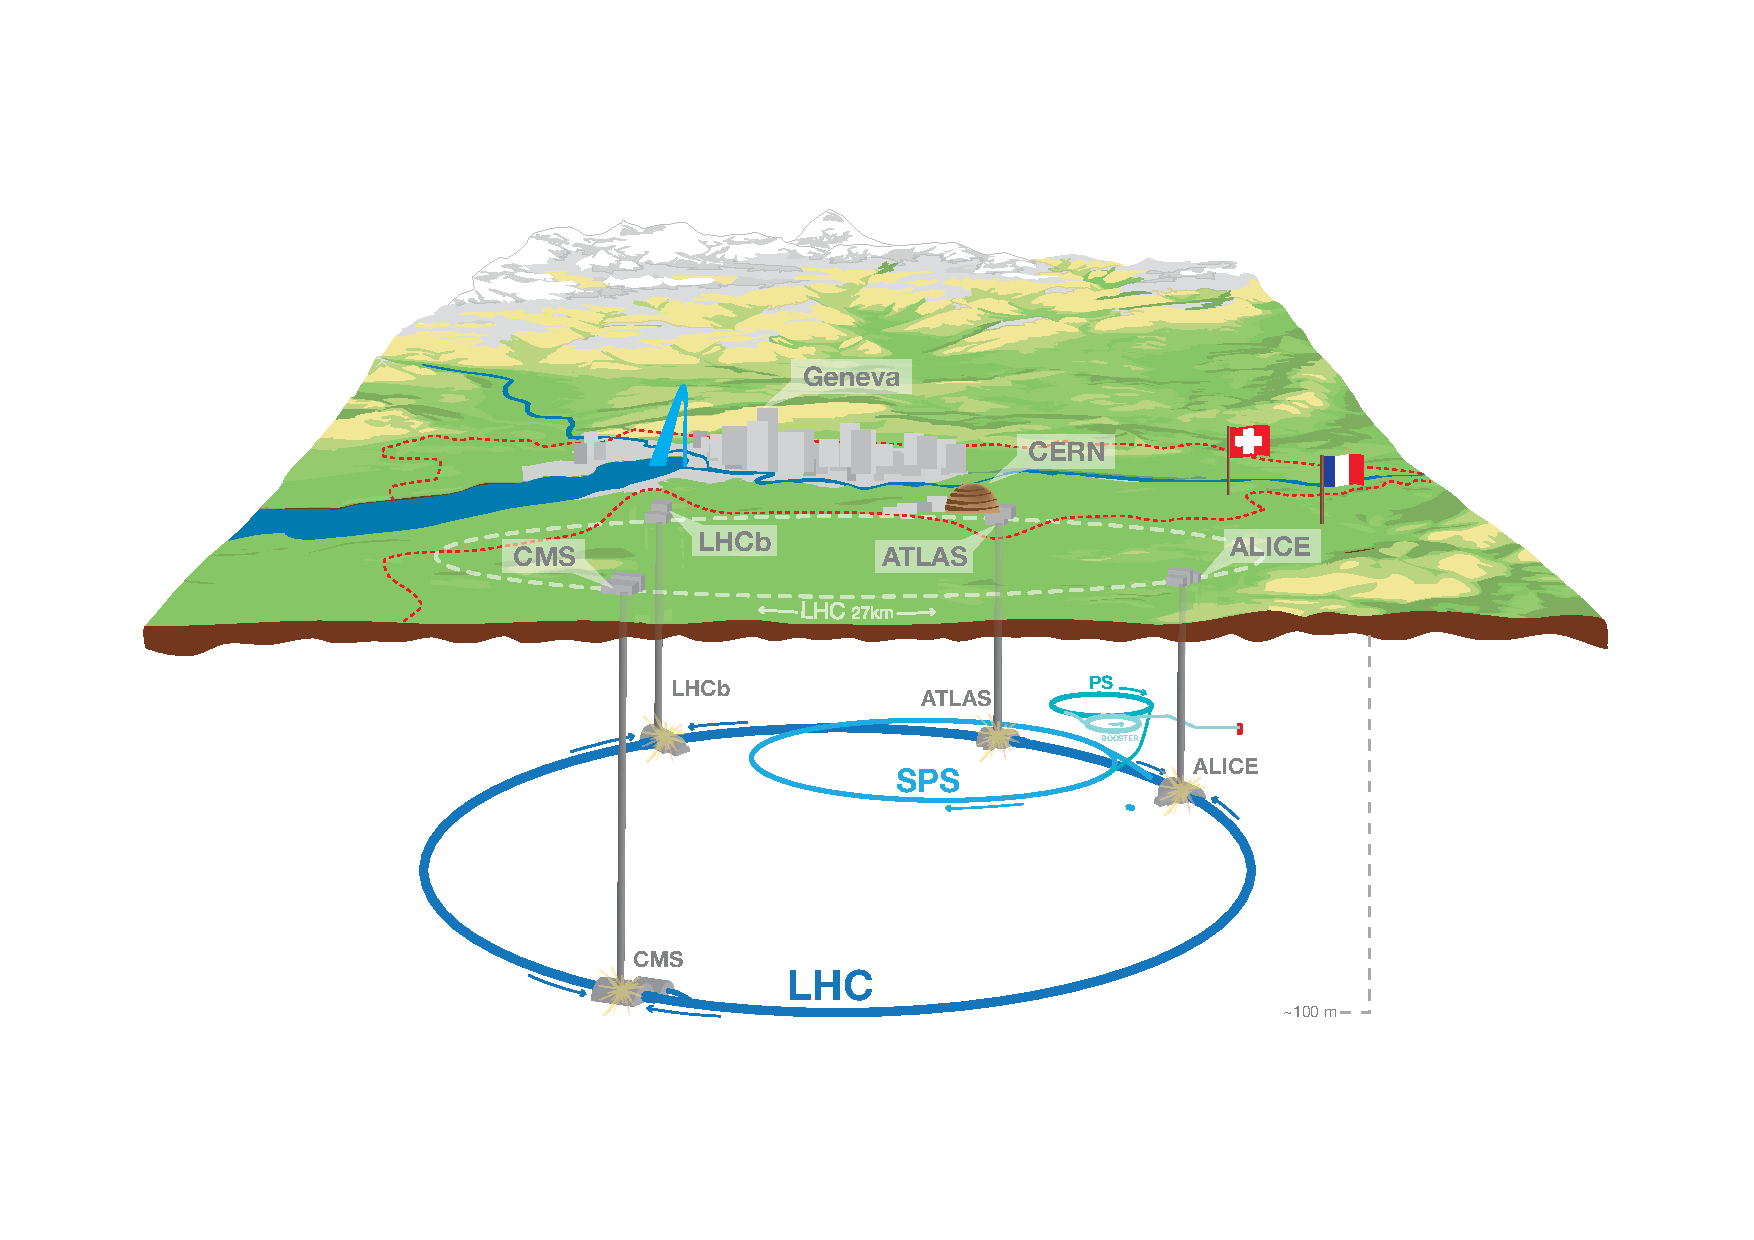
\includegraphics[width=16cm]{fig/Intro/LHCoverview.pdf}
\caption[LHC 加速器の概観]{LHC 加速器の概観\cite{cern_general_photo}}
\label{LHCoverview}
\end{figure}

図\ref{ATLASdetector}にATLAS検出器の全体像を示す。ATLAS検出器は複数の検出器で構成された大型汎用検出器で、内部飛跡検出器、カロリメーター、ミューオンスペクトロメーターという3つの検出器群で構成される。最内層に設置された内部飛跡検出器は衝突点で生じた荷電粒子の飛跡を再構成し、運動量を測定する。その外側に設置されたカロリメーターは電子、光子、ハドロンを検出しそのエネルギーを測定する。最外層に設置されたミューオンスペクトロメーターは内側の検出器を透過してきたミューオンを捉え、その運動量を測定する。これらの検出器で測定された信号をイベントごとに集約することで、陽子陽子衝突で生じた事象を再構成し、物理解析を行なっている。

\begin{figure} 
    \centering
    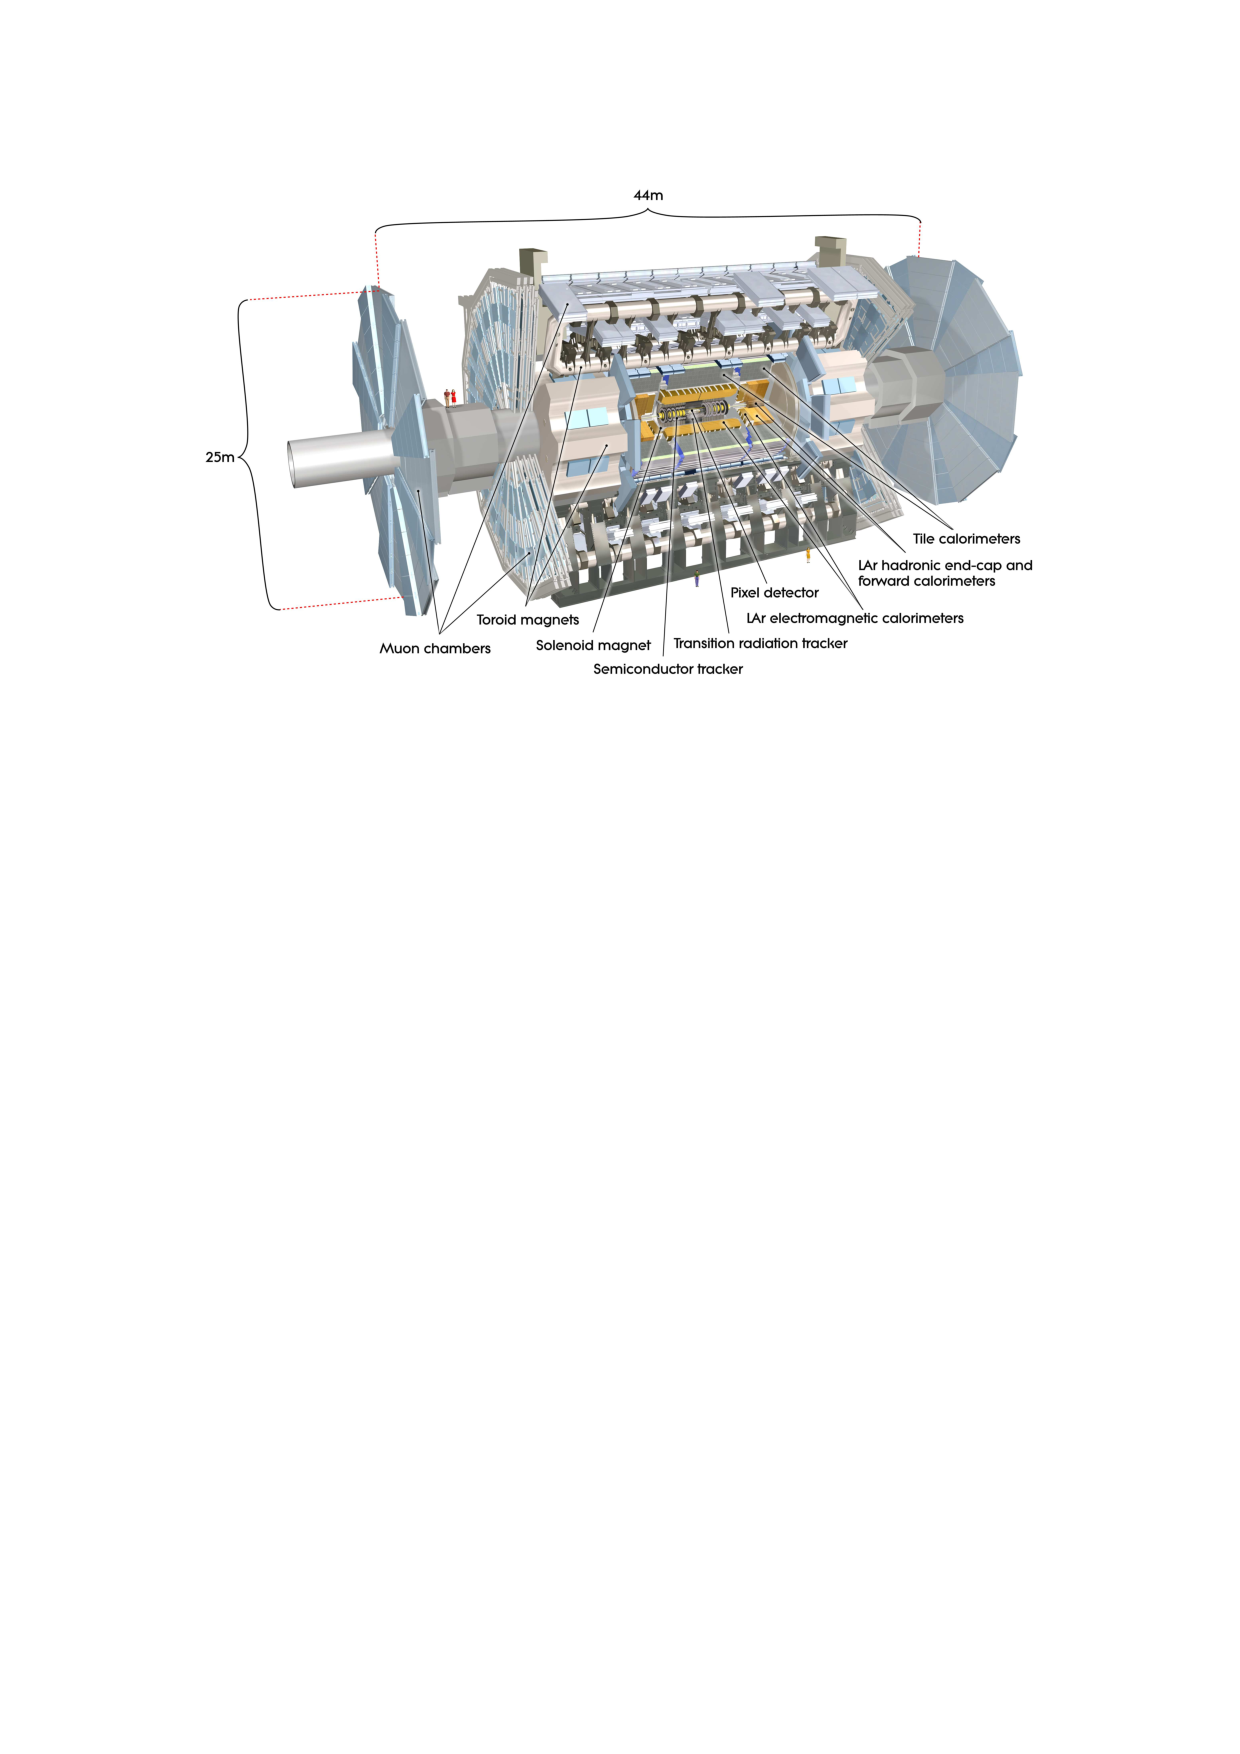
\includegraphics[width=16cm]{fig/Intro/ATLASdetector.pdf}
    \caption[ATLAS検出器の概要]{ATLAS検出器の概要図\cite{JINST:2008}}
    \label{ATLASdetector}
\end{figure}

LHC加速器内部では、陽子はおよそ$10 ^ {11}$個ずつの束にまとめられ、バンチ構造を形成する。陽子はLHCを周回しながら最大エネルギー7 TeV まで加速され、衝突点で衝突させられる。その衝突頻度は40 MHzに及ぶ。
1回のバンチ衝突で発生した大量の崩壊粒子は、それぞれの検出器にヒット信号を残す。それにより生じる情報量は1回の陽子衝突あたり約10\,Mb程度である。これは1秒間に約1 Pbpsのデータ量に相当するするため、その全てをストレージに転送し、保存することは技術的に不可能である。一方、陽子陽子衝突で生じるほとんどの事象は非弾性散乱など物理解析にとって興味の薄いものである\footnote{超対称性で予言される新粒子やヒッグス粒子の断面積は、陽子陽子衝突の全断面積より$\mathcal{O}(11)$程度小さい。}。そこでATLAS実験では莫大な背景事象の中から、興味のある事象のみを高速で選別するトリガーシステムを採用している。新粒子探索や標準模型の精密測定などの多くの解析において、統計量はその物理感度を決定する重要なパラメーターとなっている。そのため、効率的なデータ取得を実現するトリガーシステムは、物理探索に直結する重要な要素である。


% \begin{figure} 
%     \centering
%     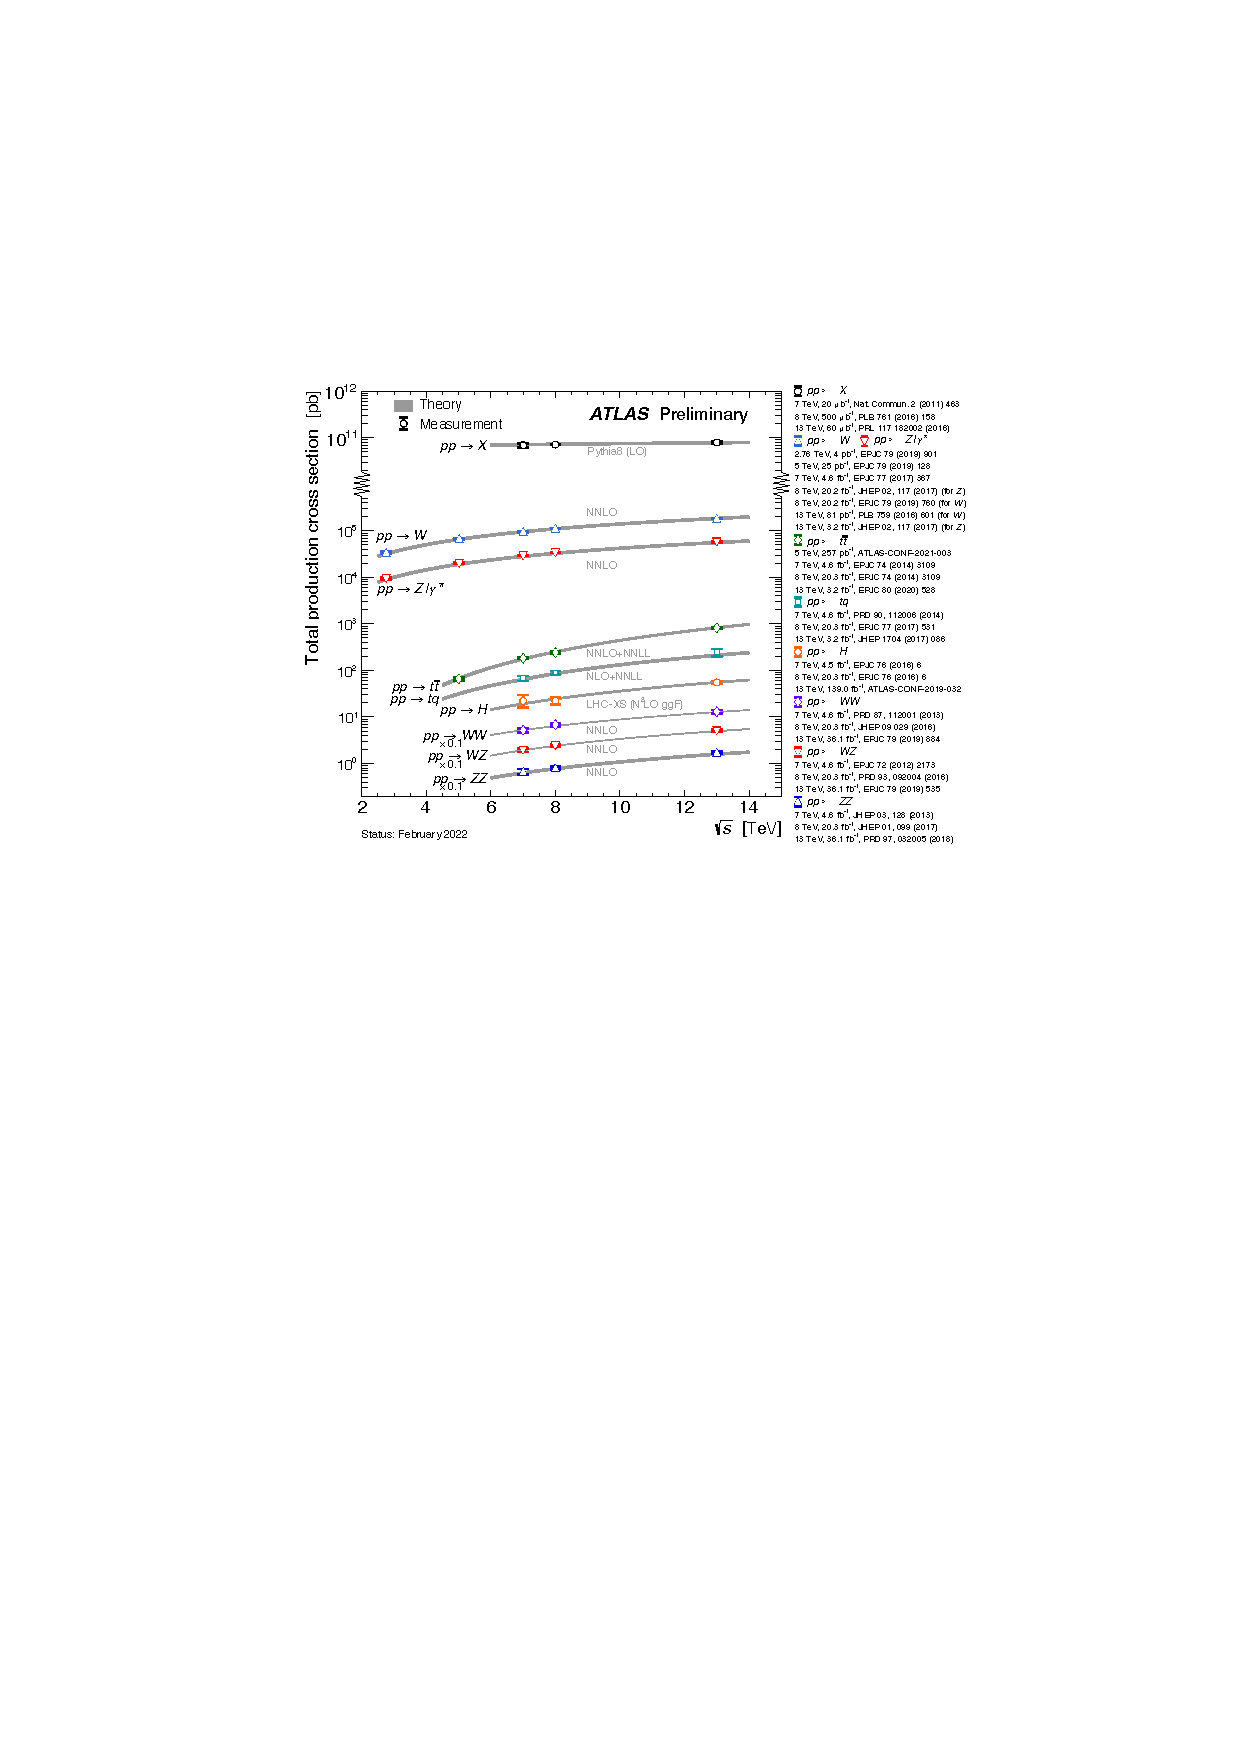
\includegraphics[width=16cm]{fig/Intro/LHCcrosssection.pdf}
%     \caption[陽子陽子衝突における各反応事象の断面積]{陽子陽子衝突における各反応事象の断面積 \cite{atlas_phys_pub_hllhc}}
%     \label{LHCcrosssection}
% \end{figure}


\section{高輝度LHC-ATLAS実験に向けたPhase-\two アップグレード}
\label{sec_intro_phase2upgrade}

\begin{figure} 
\centering
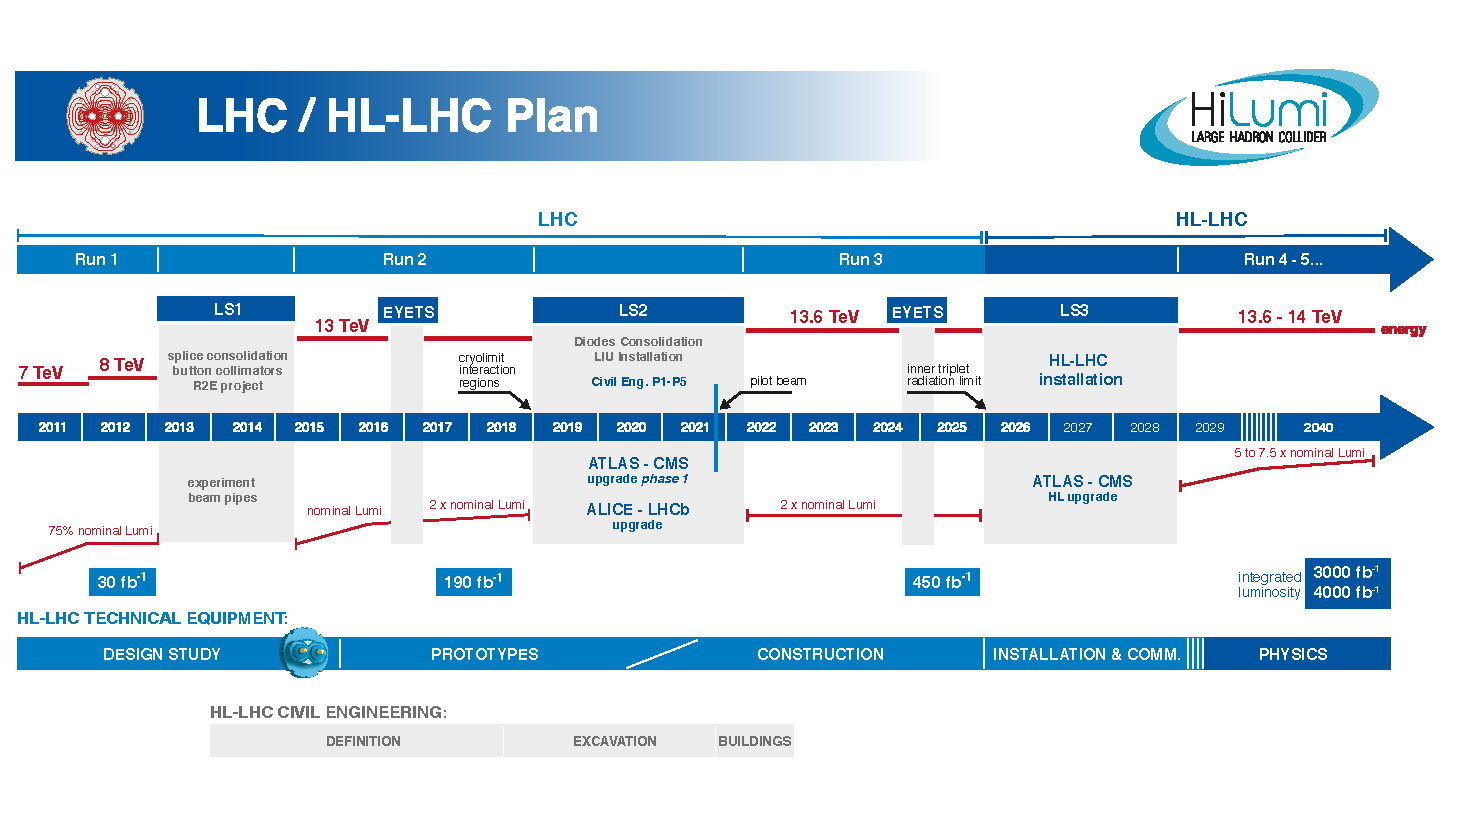
\includegraphics[width=16cm]{fig/Intro/LHCschedule.pdf}
\caption[LHC実験のスケージュール]{LHC実験のスケジュール\cite{cern_hllhc_industry}}
\label{LHCschedule}
\end{figure}

図\ref{LHCschedule}にLHCのスケジュールを示す。LHC実験は2010年から本格的に稼働し始め、2024年現在、第三期運転 (Run3) が進行中である。Run3では2025年までに累計450\,$\mathrm{fb}^{-1}$の統計量が蓄積することが予定されている。その後、3年間のLong Shutdown (LS3) を経てLHC実験は高輝度LHC実験に大幅にアプグレードされる。高輝度LHC実験では瞬間最高ルミノシティが現在の$2\times10^{34}\,\mathrm{cm}^{-2}\mathrm{s}^{-1}$から5 $\sim$ 7.5$\times10^{34}\,\mathrm{cm}^{-2}\mathrm{s}^{-1}$に増強され、2040年の実験終了までに貯められる統計量は3000  $\sim$ 4000\,$\mathrm{fb}^{-1}$に及ぶ。これにより新物理探索や標準模型の精密測定に対する感度は、大きく飛躍することが期待される。

一方で、高輝度LHC実験では瞬間ルミノシティの増加に伴い、一回のバンチ衝突ごとに発生する陽子陽子衝突数 (パイルアップ) が増加し、背景事象が大幅に増加する。これに対応するため、高輝度LHC-ATLAS実験では検出器、データ収集システム、トリガーシステムが大幅にアップグレードされる。この一連のアップグレードをPhase-\two アップグレードと呼ぶ。Phase-\two アップグレードでは、内部飛跡検出器が全てシリコン検出器に置き換わる他、各検出器のエレクトロニクスが刷新される。

本研究で扱うミューオンシステムでも、新しい検出器の増設やエレクトロニクスの刷新が行われ、背景事象と興味がある事象との判別能力が大幅に上昇する。
図\ref{Ptthreshold}に、レプトントリガーシステム (特に、電子やミューオンの横方向運動量をもとに閾値を設定するシングルレプトントリガー) のアップグレードが与える物理探索感度への影響を示す。現行のレプトンの運動量分解能や信号転送レートを維持したまま、信号事象や背景事象が増加すると、閾値を超えるレプトンの数が読み出し能力を超えるため、レプトンの横方向運動量閾値を50 GeV程度まで上げなくてはならない。対して、トリガーシステムをアップグレードしてシングルレプトンの運動量分解能向上や、読み出し能力の増強を実現することができれば横方向運動量閾値を20 GeVまで低く抑えることができる。これにより、例えば、終状態に低運動量レプトンが生成される縮退したSUSY粒子の崩壊事象へのアクセプタンスは、約4倍に増幅されることが見込まれる。

\begin{figure} 
\centering
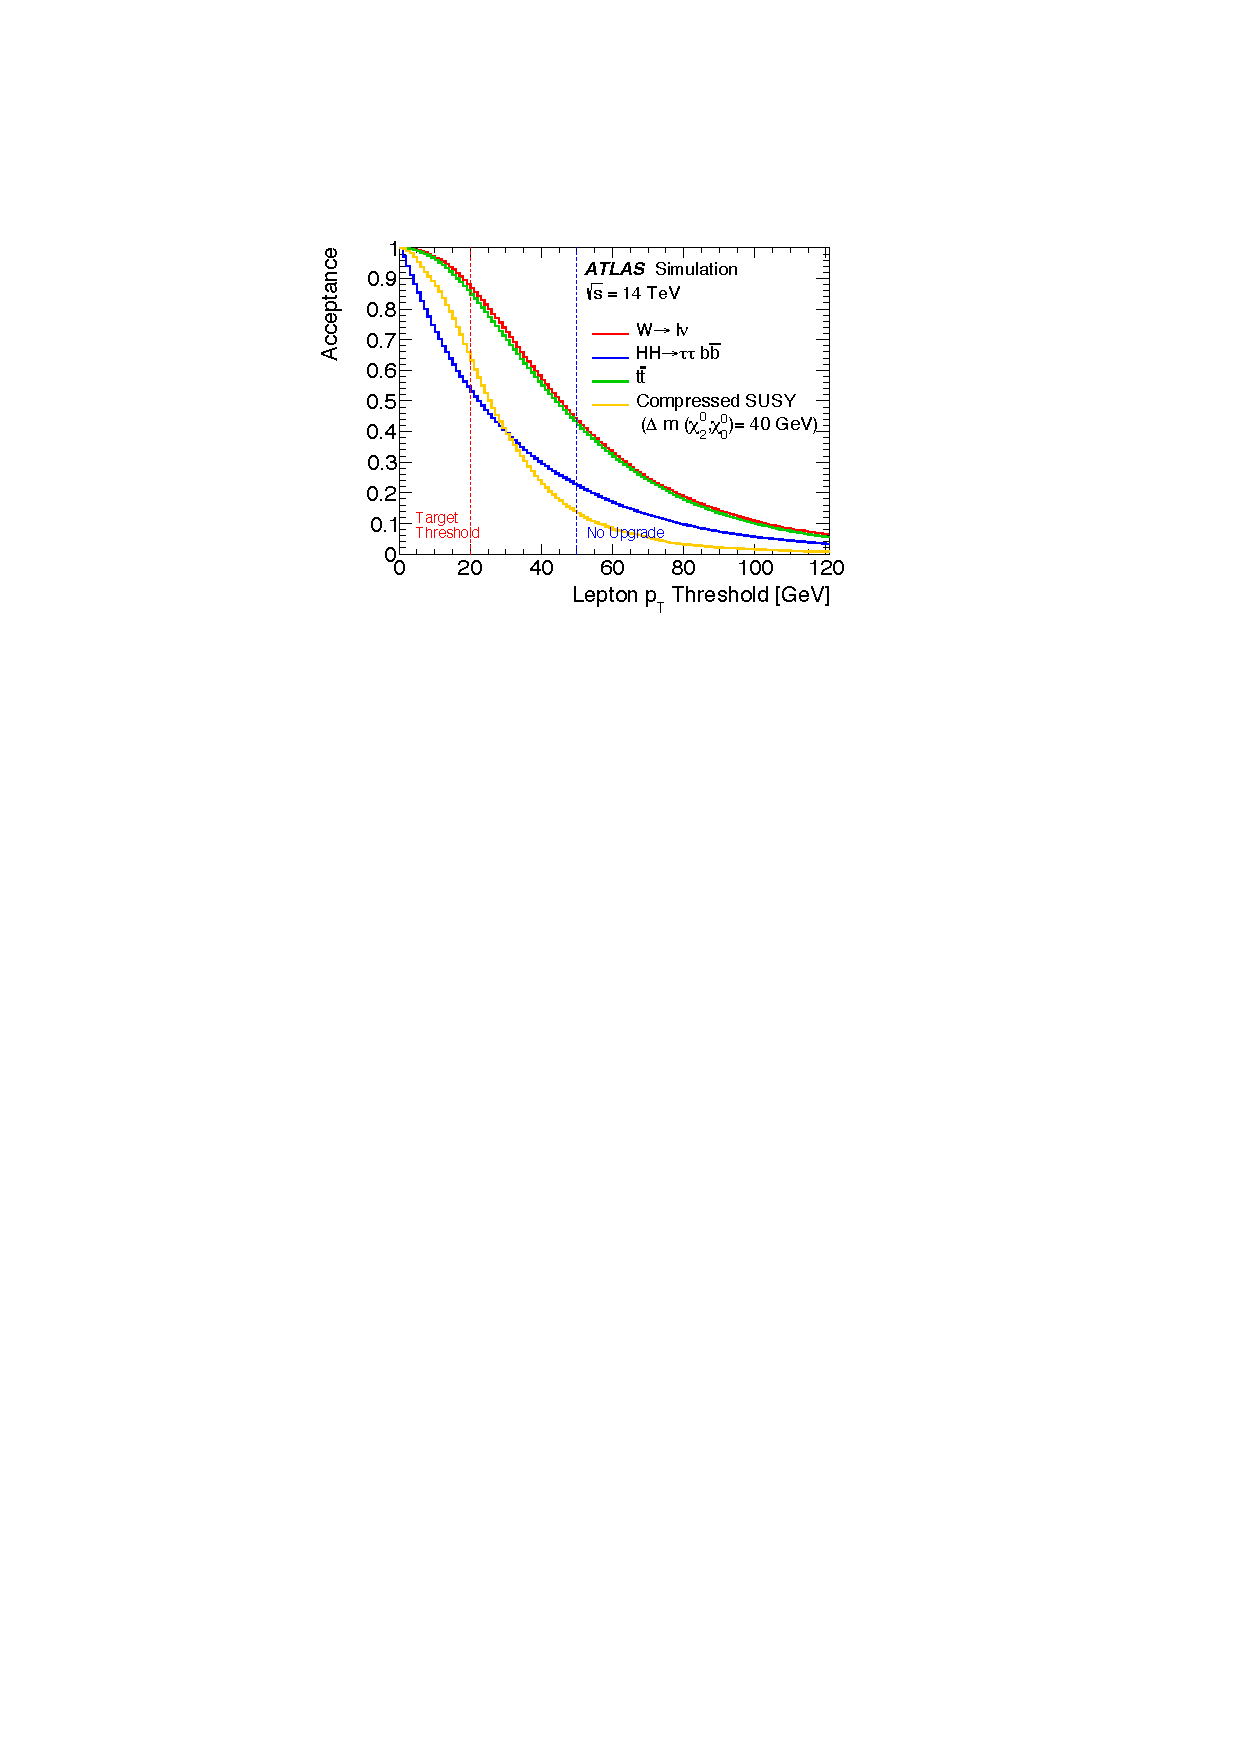
\includegraphics[width=16cm]{fig/Intro/Ptthreshold.pdf}
\caption[高輝度LHC-ATLAS実験の主なターゲットとなる事象における、レプトンの pT 閾値とアクセプタンスの関係]{高輝度LHC-ATLAS実験の主なターゲットとなる事象における、レプトンの pT 閾値とアクセプタンスの関係\cite{tdr_phase2tdaq_2017020}}
\label{Ptthreshold}
\end{figure}


\section{本論文の目的・内容と構成}
\label{sec_intro_purpose}





